\input ../SlidePreamble
\input ../preamble


\begin{document}

{\Huge
  \centerline{\bf TTIC 31230,  Fundamentals of Deep Learning}
  \vfill
  \centerline{David McAllester, Winter 2019}
  \vfill
  \centerline{\bf Pretraining}


\slide{Pretraining}

We train a model on a large data set and then either use the model as features, or fine-tune the model, on a different problem typically with a smaller training set.

\slide{Pretraining}
Pretraining can be either supervised or self-supervised.

\vfill
{\bf Supervised:} Trained on human annotations
done explicitly for the purpose of training machine learning models.  Examples include imagenet training
and training parsers on the Penn tree bank.

\vfill
{\bf Self-Supervised:} Anything not involving human annotation. Examples include language modeling (e.g. BERT) and  image colorization.

\slide{Pretraining}

Pretraining is currently essential for achieving state of the art (SOTA) performance on both NLP and vision benchmarks.

\vfill
NLP SOTA uses language modeling (self-supervised) pretraining.

\vfill
Vision SOTA still uses ImageNet pretraining, although self-supervised pretraining is making advances.

\slide{ImageNet Pretraining in Vision}

CBNet: A Novel Composite Backbone Network Architecture for Object Detection
Liu et al., Sept. 2019 (COCO leader as of February 26, 2019).

\vfill
\begin{quotation}
Generally speaking, in a typical CNN based object detector, a backbone network is used to extract basic features for detecting objects, which is usually designed for
the image classification task and pretrained on the ImageNet
dataset (Deng et al. 2009).
\end{quotation}

\slide{Instagram Pretraining, Mahajan et al., May 2018}

In our experiments, we train standard convolutional network architectures to
predict hashtags on up to 3.5 billion public Instagram images.

\vfill
To make training at this scale practical, we adopt a distributed synchronous implementation of
stochastic gradient descent with large (8k image) minibatches, following Goyal et al. 2017.

\slide{Instagram Pretraining}

\centerline{\includegraphics[width=10.0 in]{../images/InstagramPre}}

\slide{Rethinking ImageNet Pretraining, He et al., Nov. 2018}

We report competitive results on object detection and instance segmentation on the COCO dataset using standard
models trained from {\bf random initialization}.


\slide{Rethinking ImageNet Pretraining, He et al., Nov. 2018}

\centerline{\includegraphics[width=6.0 in]{../images/RethinkingPre}}

\slide{CBNet (COCO leader as of Feb, 2020)}

\centerline{\includegraphics[height=5.2 in]{\images/CBNet}}


\slide{CBNet (COCO leader as of Feb, 2020)}

\begin{quotation}
We initialize each assembled backbone of CBNet with the pretrained model of the single backbone which is widely and
freely available today, such as ResNet and ResNeXt
\end{quotation}

\slide{}

\centerline{\bf Self-Supervised Feature Learning for Vision}

\vfill
\vfill

\slidetwo{Learning Representations for Colorization}{Larsson et al., 2016}

\vfill
\centerline{\includegraphics[width = 5in]{../images/colorizationGreg2}}
\centerline{$x$ \hspace{4em} $y_\Phi(x)$ \hspace{4em} $y$}

\vfill
Trained to minimize $L_2$ image distortion between $y_\Phi(x)$ and $y$.

\slide{Evaluation}

Self-supervised representations (features) are tested by training a {\color{red} linear} classifier for ImageNet.

\slidetwo{Self-Supervised Pretraining in Vision}{Feature Learning by Inpainting, Pathak et al., 2016}

\centerline{\includegraphics[width = 3in]{../images/LearnRepInpa}}

Trained to minimize distortion between $y_\Phi(x)$ and $y$ and to {\color{red} maximize} discriminator loss for distinguishing $y_\Phi(x)$ from $y$.

\slide{Contrastive Predictive Coding (CPC)}

We consider a population distribution on pairs $\tuple{x,y}$.

\vfill
For example $x$ and $y$ might be video frames separated by 10 seconds in a video.

\vfill
For simplicity we will assume that the marginal distributions on $x$ and $y$ are the same --- the probability that an image occurs as a first frame
is the same as the probability that image occurs as a second frame.

\vfill
In CPC we draw a pair $\tuple{x,y}$ and {\color{red} minimize} a discriminator loss for distinguishing $z_\Phi(y)$ from $z_\Phi(\tilde{y})$ for $\tilde{y} \sim \pop(y)$.
The discriminator gets to see $x$.

\slide{Contrastive Predictive Coding (CPC)}

For $N \geq 2$ let  $\tilde{P}^{(N)}$ be the distribution on tuples $\tuple{i,y_1,\ldots,y_N,x}$
defined by the following process.

\begin{itemize}
\item draw a pair $\tuple{x,y}$ from the population.

\item drawn a sequence of $N-1$ ``distractor values'' from the marginal distribution $\pop(y)$.  These are unrelated to $x$.

\item insert $y$ at a random position among the distractors to get the sequence
$y_1,\ldots,y_N$.

\item return the tuple $\tuple{i,y_1,\ldots,y_N,x}$ where $i$ is the index of $y$ among the distractors.
\end{itemize}

\slide{Contrastive Predictive Coding (CPC)}

\begin{eqnarray*}
\Phi^*  & = & \argmin_\Phi\;{\cal L}_\mathrm{CPC}(\Phi) \\
\\
{\cal L}_\mathrm{CPC}(\Phi) &= & E_{\tuple{i,y_1,\ldots,y_N,x} \sim \tilde{P}^{(N)}} \\
\\
& & ~\;\;\;\;\;\; -\ln P_\mathrm{CPC}(i|z_\Phi(y_1),\ldots,z_\Phi(y_N),z_\Phi(x))
\end{eqnarray*}

\vfill
$$P_\mathrm{CPC}(i|z_1,\ldots,z_N,z_x) = \softmax_i\;z_i^\top z_x$$

\slide{Contrastive Predictive Coding (CPC)}

\begin{eqnarray*}
\Phi^*  & = & \argmin_\Phi\;{\cal L}_\mathrm{CPC}(\Phi)
\end{eqnarray*}

\vfill
$$P_\Phi(i|z_1,\ldots,z_n,z_x) = \softmax_i\;z_i^\top z_x$$

\vfill
As $N$ gets larger the contrastive discrimination task gets harder.

\vfill
The task is also made difficult by the requirement that the score is defined to be an inner product of feature vectors.

\slide{Contrastive Predictive Coding (CPC)}

(SimCLR:) A Simple Framework for Contrastive Learning of Visual Representations, Chen et al., Feb. 2020 (self-supervised leader as of February, 2020).

\vfill
They use a distribution on pairs $\tuple{x,y}$ defined by drawing an image $s$ from ImageNet and then drawing $x$ and $y$ as random ``augmentations'' (modifications) of the image $s$
--- either a random translation, rotation, color jitter, masking, edge image, or a composition of these modifications.

\slide{Contrastive Predictive Coding (CPC)}

The feature map $z_\Phi$ can then be applied to the images of ImageNet.

\vfill
The feature map $z_\Phi$ is then tested by using a {\color{red} linear} classifier for ImageNet based on these features.

\slide{SimCLR}

\centerline{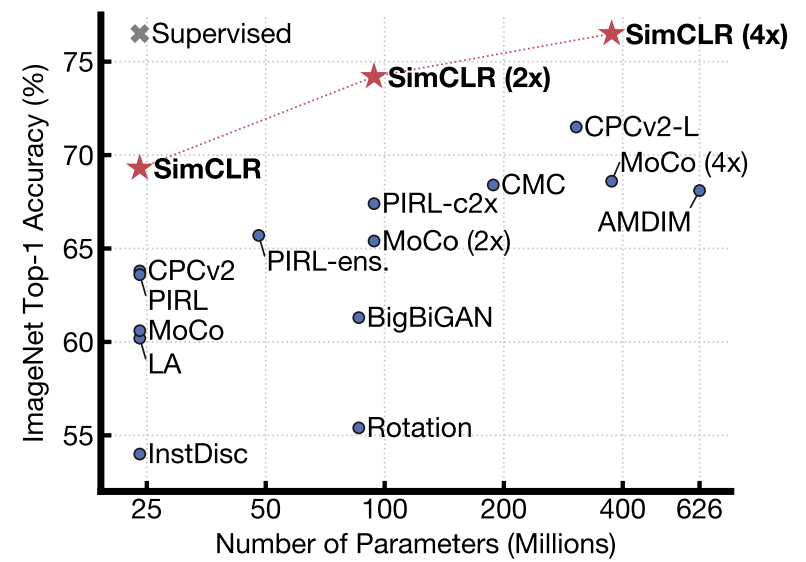
\includegraphics[height=5.2 in]{\images/SimCLR}}

\slide{Mutual Information Objectives}

CPC represents a fundamental shift in the self-supervised training objective.

\vfill
GANs and VAEs are motivated by modeling $\pop(y)$.

\vfill
But in CPC there is no attempt to model $\pop(y)$.

\vfill
CPC can be viewed as training a feature map $z_\Phi$ so as to maximize the mutual information {\color{red} $I(z_\Phi(x),z_\Phi(y))$} while, at the same time, making $z_\Phi(x)$ useful
for linear classifiers.

\slide{Relationship to Noise Contrastive Estimation}

CPC is noise contrastive estimation (NCE) with ``noise'' generated by drawing $y$ unrelated to $x$.
By the NCE theorems, universality implies

$$P_{\Phi^*}(i|z_1,\ldots,z_N,z_x) = \softmax_i \;\ln \frac{\pop(z_i|z_x)}{\pop(z_i)}$$

and also

{\huge
\begin{eqnarray*}
{\cal L}_\mathrm{CPC} & \geq & \ln N - \frac{N-1}{N}(KL(\pop(z_y|z_x),\pop(z_y)) + KL(\pop(z_y),\pop(z_y|z_x))) \\
\\
& = & \ln N - \frac{N-1}{N}({\color{red} I(z_x,z_y)} + KL(\pop(z_y),\pop(z_y|z_x)))
\end{eqnarray*}
}

\slide{Deep Co-Training}

For a population on $\tuple{x,y}$ and a ``feature map'' $z_\Phi$ we optimize $\Phi$ by

\vfill
$$\Phi^* = \argmax_\Phi \; I(z_\Phi(x),z_\Phi(y)) - \beta H(z_\Phi(x))$$


\vfill
Here we can think of $z_\Phi(x)$ as what we remember about a past $x$ to carry information about a future $y$ while maintaining low memory requirements.

\slide{Deep Co-Training}

\begin{eqnarray*}
\Phi^* & = & \argmax_\Phi \; (1-\beta)\hat{H}_\Phi(z_\Phi(x)) - \hat{H}_\Phi(z_\Phi(x)|z_\Phi(y)) \\
\\
\hat{H}_\Phi(z_\Phi(x)) & = & E_x \; -\ln \;P_{\Psi^*(\Phi)}(z_\Phi(x)) \\
\\
\Psi^*(\Phi) & = & \argmin_\Psi\;E_x\;-\ln P_\Psi(z_\Phi(x)) \\
\\
\hat{H}_\Phi(z_\Phi(x)|z_\Phi(y)) & = & E_{x,y} \; -\ln P_\Phi(z_\Phi(x)|z_\Phi(y)) 
\end{eqnarray*}

\vfill
Here, as in CPC, we only model distributions on $z$.  There is no attempt to model distributions on $x$ or $y$.

\slide{Pretraining for NLP}

Unlike vision, in NLP self-supervised pretraining is now required for strong benchmark performance.

\vfill

\slide{Moore's Law of AI: Natural Language Understanding}

GLUE: General Language Understanding Evaluation

\vfill

\centerline{\normalsize ArXiv 1804.07461}
\centerline{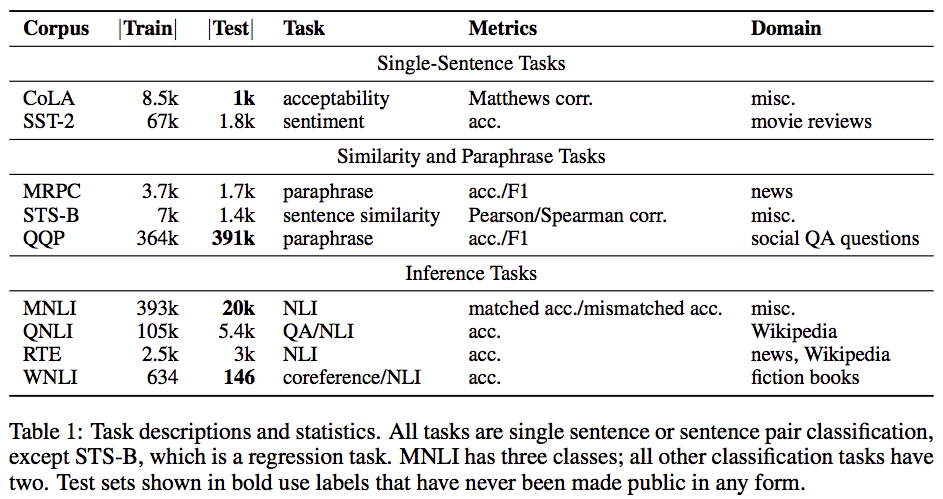
\includegraphics[width= 7in]{\images/GLUE}}

\slide{GLUE Leader Board as of February 27, 2020}

\centerline{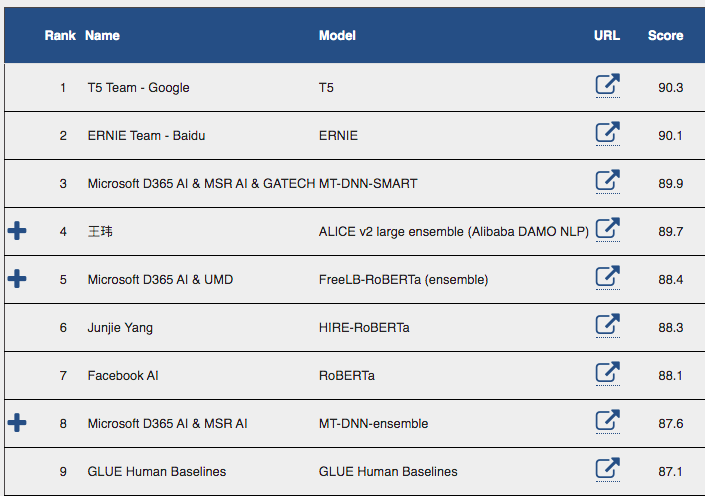
\includegraphics[width= 7in]{\images/GLUELeader}}

\slide{SuperGLUE Leader Board as of February 27, 2020}

\centerline{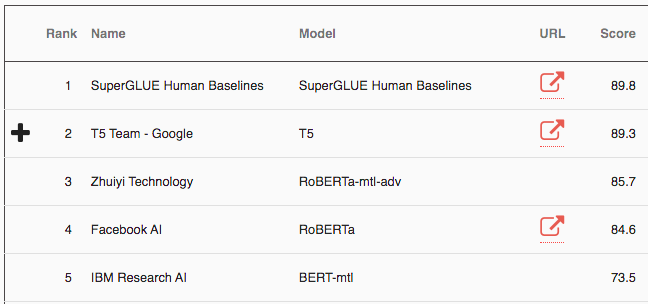
\includegraphics[width= 9in]{\images/SuperLeader}}


\slide{Pretrained Word Embeddings}

Advances in Pre-Training Distributed Word Representations, Mikolov et al., 2017

\vfill
We want a mapping from a word $w$ to a vector $e(w)$ --- a word embedding.

\vfill
{\color{red} fastText} from Facebook is currently popular.

\vfill
It provides both contextual bag of words (cbow) and byte pair encoding (BPE) word vectors.

\slide{cbow word vectors}

We construct a population distribution on pairs $(c,w)$ here $c$ is a bag of word context and $w$ is a word.

\vfill
$$\Phi^* = \argmin_\Phi E_{c,w}\;-\ln P(w|c)$$

\vfill
$\Phi$ consists of a matrix $e[w,i]$ where $e[w,I]$ is the word embedding of $w$, and a matrix $e'[w,i]$ giving the embedding of the word
$w$ when it appears in a context.

\vfill
A score $s(w|c)$ is defined by
$$s(w|c) = \frac{1}{|c|} \sum_{w' \in c}\;e(w)^\top e'(w')$$

\slide{Negative Sampling in cbow}

\vfill
Rather than define $P_\Phi(w|c)$ by a softmax over $w$, one uses restricted negative sampling.

\vfill
We construct a training set of triples $(w,c,N_C)$

\vfill
$$\Phi^* = \argmin_\Phi\;E_{w,c,N_c}\;\ln\left(1 + e^{-s(w,c)}\right) + \sum_{n \in N_C} \ln\;\left(1 + e^{s(n,c)}\right)$$

\slide{Byte Pair Encoding (BPE)}

BPE constructs a set of character n-grams by starting with the unigrams and then greedily merging most common bigrams of n-grams.

\vfill
Given a set of character n-grams each word is treated as a bag of character n-grams.

\vfill
$$e[w] = \frac{1}{N} \sum_{n \in w}\; e(n)$$

\vfill
Current systems use byte pairs but train the byte pair embeddings as part of transformer training.

\slide{The Transformer}

Attention is All You Need, Vaswani et al., June 2017

\vfill
The transformer is like an RNN in that it takes a sequence of words and converts it to a sequence of vectors.

\vfill
The output vectors are sometimes called contextual word embeddings.

\vfill
But unlike RNNs, transformers run in parallel time in proportion to the layering depth
independent of the length of the block.

\slide{The Transformer}

\centerline{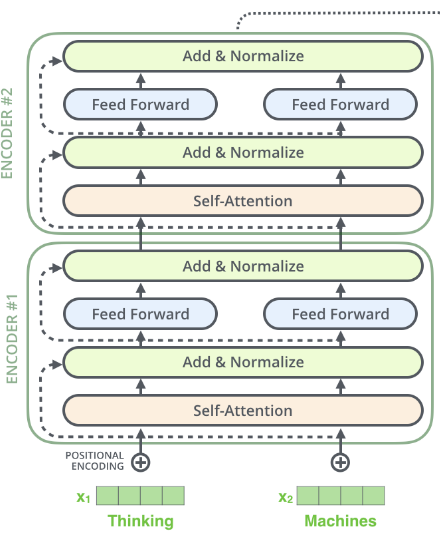
\includegraphics[height=4.5in]{\images/transformer}}

{\huge
\centerline{Jay Alammar's blog}
}

All layers run in $O(1)$ time independent of block length.

\slide{A Self-Attention Layer}

Given an $h_\mathrm{in}[T,J]$ we will construct $h_\mathrm{out}[T,J]$
\vfill

We first construct a head-specific self-attention $\alpha[k,t_1,t_2]$ --- the attention position
$t_1$ is giving to position $t_2$ for head $k$.

\vfill
\centerline{\includegraphics[height  = 3.5in]{../images/Transformera}}

\slide{Computing the Self Attention}

For each head $k$ and position $t$ we compute a key vector and a query vector with dimension $U$ typically smaller than dimension $J$.
      
\begin{eqnarray*}
\mathrm{Query}[k,t,U] & = & W^Q[k,U,J]h_\mathrm{in}[t,J] \\
\\
\mathrm{Key}[k,t,U] & = &  W^K[k,U,J]h_\mathrm{in}[t,J] \\
\\
\alpha[k,t_1,t_2] & = & \softmax_{t_2}\; \mathrm{Query}[k,t_1,U]\mathrm{Key}[k,t_2,U]
\end{eqnarray*}

\slide{Computing the Output}

We require $I = J/K$.
      
\begin{eqnarray*}
\mathrm{Value}[k,t,I] & = & W^V[k,I,J]h_\mathrm{in}[t,J] \\
\\
\mathrm{Out}[k,t,I] & = & \sum_{t'}\alpha[k,t,t']\mathrm{Value}[k,t',I] \\
\\
h_\mathrm{out}[t,J] & = & \mathrm{Out}[1,t,I];\cdots;\mathrm{Out}[K,t,I]
\end{eqnarray*}

\slide{The Transformer}

\centerline{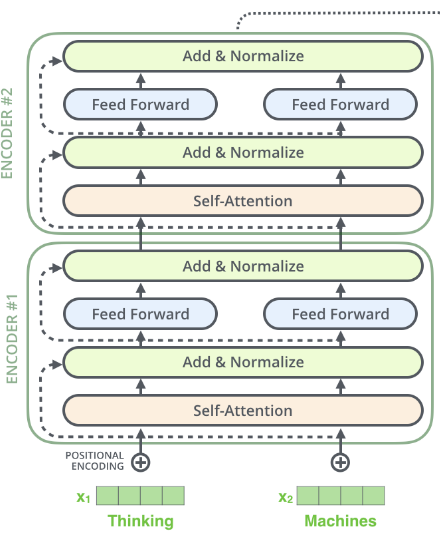
\includegraphics[height=4.5in]{\images/transformer}}

{\huge
\centerline{Jay Alammar's blog}
}

Position encodings are inserted at the bottom.

\slide{Encoding Positional Information}

At the input layer we augment the word embeddings with position information. For example:

\vfill
{\color{red} $$h[0,t,J] = e[w[t],I];e^{i\omega t}\;;e^{i2\omega t}\;;e^{i4\omega t}\cdots;e^{i2^k\omega t}$$}

\vfill
In modern versions there is a position encodings trained for each position in the block.

\slide{ELMO: Language Modeling}

To do language modeling we fix $\alpha[k,t_1,t_2] = 0$ for $t_2 > t_1$.

\vfill
We can then predict the word $w[t+1]$ as

\vfill
$$P(w_{t+1}|w_1,\ldots,w_t) = \softmax_w\;e[w,I]h_\mathrm{top}[t,I]$$

\slide{Machine Translation}

Translation is just a conditional language model.

\vfill
We take the input English sentence followed by a special token and then generate from the transformer language model.

\slide{Continuing from a Prompt}


GPT-2 from Open AI.

\vfill
{\color{red} Continue from:}

\vfill
In a shocking finding, scientist discovered a herd of unicorns living in a remote, previously unexplored valley, in the Andes Mountains. Even more surprising to the researchers was the fact that the unicorns spoke perfect English.

\slide{The Predicted Continuation}

{\color{red} Continuation excerpted from a single response, the response selected from 10 tries.}

\bigskip

The scientist named the population, after their distinctive horn, Ovid’s Unicorn. These four-horned, silver-white unicorns were previously unknown to science.

Now, after almost two centuries, the mystery of what sparked this odd phenomenon is finally solved.

Dr. Jorge Pérez, an evolutionary biologist from the University of La Paz, and several companions, were exploring the Andes Mountains when ...
Pérez and his friends were astonished to see the unicorn herd. ...
While examining these bizarre creatures the scientists discovered that the creatures also spoke some fairly regular English. Pérez stated, “We can see, for example, that they have a common ‘language,’ something like a dialect or dialectic.”

Dr. Pérez believes that the unicorns may have originated in Argentina ... some believe that perhaps the creatures were created when a human and a unicorn met each other in a time before human civilization. ... However, Pérez also pointed out that it is likely that the only way of knowing for sure if unicorns are indeed the descendants of a lost alien race is through DNA. ...

\slide{Fine Tuning on Question Answering}

COMET: Busselut et al, June 2019.

\vfill
Charlie is drifting though life:

\centerline{\includegraphics[height=4in]{\images/COMET}}\

\slide{The Chatbot Meena}

\centerline{\includegraphics[height=4in]{\images/meena1}}\

\slide{The Chatbot Meena}

\centerline{\includegraphics[height=4in]{\images/meena2}}\

\slide{BERT: Blank Languagage Modeling}

We replace a random subset of the words with a blank token.

\vfill
We run a transformer on a block of text containing some blanks.

\vfill
For a blank occurring at position $t$ we predict the word at position $t$:

\vfill
$$P(w) = \softmax_w\;h[t,J]e[w,J]$$

\vfill
Blank language modeling outperforms language modeling when used for pretraining in classification tasks such as the GLUE tasks.

\slide{GLUE Leader Board as of February 27, 2020}

\centerline{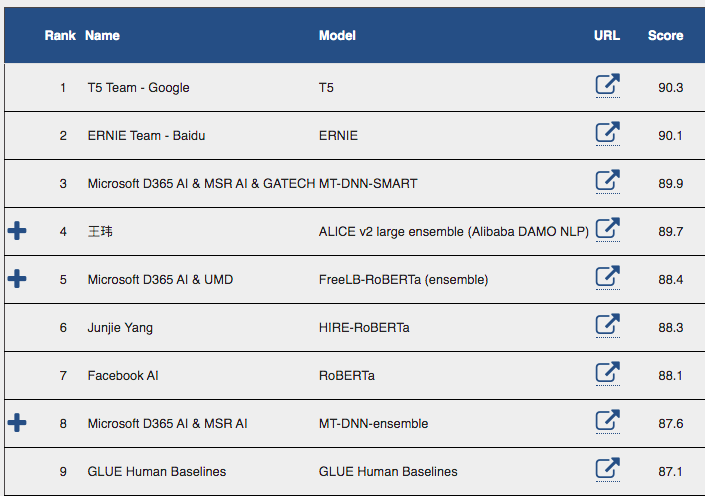
\includegraphics[width= 7in]{\images/GLUELeader}}


\slide{END}

}
\end{document}
